\documentclass[11pt,a4paper]{article}
\usepackage{tikz}
\usetikzlibrary{arrows.meta,positioning}
\usepackage{tabularx}
\usepackage{amsmath,amssymb,amsthm}
\usepackage{geometry}
\geometry{margin=1in}
\usepackage{hyperref}
\usepackage{graphicx}
\usepackage{setspace}
\onehalfspacing

\title{\textbf{Paper F-05: Plasma Dynamics:\\ A Constraint-Driven Flux Dynamics (CDFD) Perspective}}
\author{Steve Bico Mujjabi, MD\\
\small Independent Researcher\\
\small Founder, Vura Labs\\
\small Kampala, Uganda\\
\small ORCID: 0009-0001-0556-5516}
\date{August 2026}

\begin{document}
\maketitle

% BEGIN SHARED-METHODS POINTER
\noindent\textit{Shared Part IV notation and evidence boundaries are defined in \path{PART_IV_METHODS_AND_CLAIM_BOUNDARY.md}. This paper states only its local observables, comparison, and failure conditions.}
% END SHARED-METHODS POINTER


\begin{abstract}
This paper develops a falsifiable CDFD/AFL model of Plasma Dynamics. It maps particles, heat, current, radiation, and momentum to driving flux $\Phi$, fields, collisions, geometry, confinement, and transport barriers to active constraint $C$, waves, reconnection, turbulence, control, and profile adjustment to responsiveness $S$, and magnetic topology, distribution functions, impurities, and prior events to structural memory $M_s$. The target outcome is confinement, heating, instability, transport, and recovery, tested against laboratory diagnostics, solar observations, in-situ spacecraft data, and simulations. The paper treats universality as a shared model architecture rather than an assertion that unlike systems have the same material mechanism. It states the negative result that would make the mapping unnecessary and places the domain claim inside the cumulative CDFD programme and its reproducible runtime boundary.
\end{abstract}

\section{Introduction}

Plasma is the most abundant form of ordinary matter in the universe, constituting stellar interiors, solar coronas, and the interstellar medium. Unlike neutral gases, plasmas are exquisitely sensitive to electromagnetic fields. The concept of "magnetic flux freezing" dictates that in an ideal, perfectly conducting plasma, magnetic field lines are "frozen" into the fluid and must move with it.

However, non-ideal plasmas undergo magnetic reconnection---a violent topological rearrangement of the field lines that releases massive amounts of energy. Traditional MHD requires localized resistivity anomalies to explain this. In the Constraint-Driven Flux Dynamics (CDFD) framework, reconnection is represented as. It is a universal systemic response to constraint locking.

\section{The Plasma Surface and Magnetic Memory}
We define the plasma flow utilizing the Adaptive Operating Ratio:
\begin{equation}
    \Psi_s = \left( \frac{\Phi}{C} \right) \cdot S \cdot M_s
\end{equation}

For a highly conductive plasma (e.g., the solar corona or a fusion tokamak), the components map as follows:
\begin{itemize}
    \item \textbf{Flux ($\Phi$)}: The kinetic flow of the plasma fluid and the associated electrical currents ($J$).
    \item \textbf{Constraint ($C$)}: The Lorentz force ($\mathbf{J} \times \mathbf{B}$) and the tension of the magnetic field lines. The field topology resists the natural expansion or shear of the fluid flow.
    \item \textbf{Responsiveness ($S$)}: The ionization fraction and the thermal capacity of the plasma, defining its ability to conduct current.
    \item \textbf{Memory ($M_s$)}: Magnetic helicity and flux freezing. The fact that the plasma cannot cross field lines means it "remembers" its initial topology. This creates a rigid structural memory.
\end{itemize}

\subsection{Constraint Locking and Magnetic Reconnection}
As the plasma flows (e.g., driven by solar convective granules), it twists and shears the frozen-in magnetic field lines. This increases the magnetic tension. In CDFD terms, the continuous flux $\Phi$ is accumulating a massive topological constraint $C$.

Because the plasma has perfect memory ($M_s \to 1.0$, due to flux freezing), it cannot smoothly adapt. The constraint $C$ grows exponentially, while the effective throughput bottlenecks. The system's life number plummets: $\Psi_s \ll 1$.

At this point, the plasma has entered a chronic constraint state, exactly analogous to a diseased biological tissue suffering from chronic ischemia. The system is structurally unstable. To prevent total stagnation, the system undergoes magnetic reconnection. The magnetic memory ($M_s$) is instantaneously erased at the reconnection X-point. The topological constraint $C$ snaps, and the stored constraint energy is violently dumped back into the system as kinetic flow $\Phi$.



\section{Measurement Layer}

% BEGIN PART IV MAJOR CROSS-DOMAIN UPGRADE
\section{Cross-Domain Model Upgrade: Mechanism, Scale, and Tests}

\subsection{Observable Translation}

The paper-specific translation begins with an observable chain rather than a
verbal analogy. For Plasma Dynamics, the proposed drive is particles, heat, current, radiation, and momentum.
The active limitation is fields, collisions, geometry, confinement, and transport barriers. Responsiveness is carried by
waves, reconnection, turbulence, control, and profile adjustment, while retained state is represented by
magnetic topology, distribution functions, impurities, and prior events. The outcome to explain is confinement, heating, instability, transport, and recovery.

\begin{table}[htbp]
\centering
\small
\caption{Operational CDFD/AFL map for Paper F-05.}
\begin{tabularx}{\textwidth}{|l|X|X|}
\hline
\textbf{Term} & \textbf{Paper-specific observable meaning} & \textbf{Measurement question} \\
\hline
$\Phi$ & particles, heat, current, radiation, and momentum & What rate, load, gradient, or demand enters the focal system? \\
\hline
$C$ & fields, collisions, geometry, confinement, and transport barriers & Which measured bottleneck limits transfer, function, or recovery? \\
\hline
$S$ & waves, reconnection, turbulence, control, and profile adjustment & Which process changes effective capacity or reroutes the load? \\
\hline
$M_s$ & magnetic topology, distribution functions, impurities, and prior events & Which retained state makes equal present loads produce different futures? \\
\hline
$Y$ & confinement, heating, instability, transport, and recovery & Which outcome is predicted out of sample, with uncertainty? \\
\hline
\end{tabularx}
\end{table}

\begin{figure}[htbp]
\centering
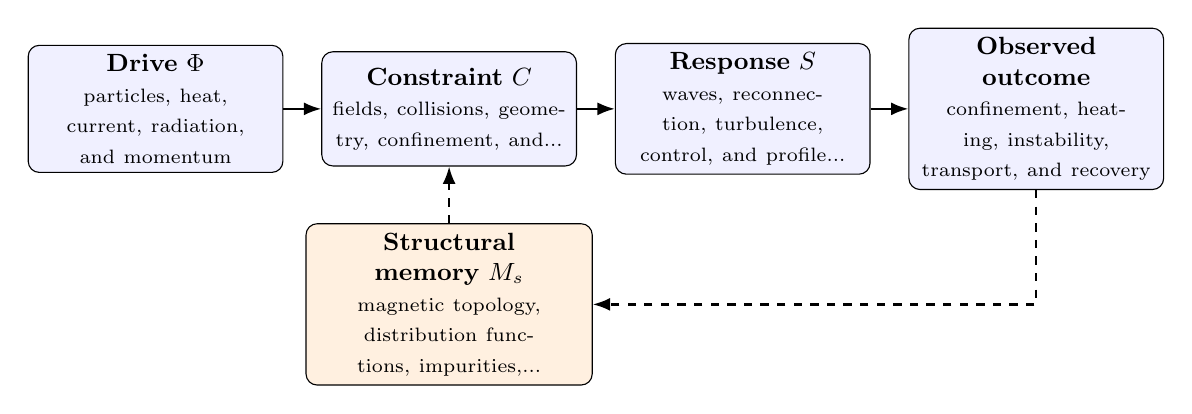
\begin{tikzpicture}[
    node distance=0.48cm,
    every node/.style={font=\small},
    box/.style={draw, rounded corners, align=center, minimum height=1.45cm, text width=3.0cm, fill=blue!6},
    memory/.style={draw, rounded corners, align=center, minimum height=1.25cm, text width=3.4cm, fill=orange!12},
    flow/.style={-{Latex[length=2.2mm]}, thick},
    feedback/.style={-{Latex[length=2.2mm]}, thick, dashed}
]
\node[box] (drive) {\textbf{Drive $\Phi$}\\\scriptsize particles, heat, current, radiation, and momentum};
\node[box, right=of drive] (constraint) {\textbf{Constraint $C$}\\\scriptsize fields, collisions, geometry, confinement, and...};
\node[box, right=of constraint] (response) {\textbf{Response $S$}\\\scriptsize waves, reconnection, turbulence, control, and profile...};
\node[box, right=of response] (outcome) {\textbf{Observed outcome}\\\scriptsize confinement, heating, instability, transport, and recovery};
\node[memory, below=0.72cm of constraint] (memory) {\textbf{Structural memory $M_s$}\\\scriptsize magnetic topology, distribution functions, impurities,...};
\draw[flow] (drive) -- (constraint);
\draw[flow] (constraint) -- (response);
\draw[flow] (response) -- (outcome);
\draw[feedback] (outcome.south) |- (memory.east);
\draw[feedback] (memory.north) -- (constraint.south);
\end{tikzpicture}
\caption{Paper F-05 observable CDFD/AFL architecture for Plasma Dynamics. Solid arrows give the proposed forward chain; dashed arrows make history-dependent feedback explicit.}
\label{fig:f05-architecture}
\end{figure}

\subsection{Paper-Specific Causal Hypothesis}

For this paper, the hypothesized causal sequence is specific. A change in
particles, heat, current, radiation, and momentum arrives faster than waves, reconnection, turbulence, control, and profile adjustment can compensate.
This raises or redistributes fields, collisions, geometry, confinement, and transport barriers. If the load persists,
the retained state encoded by magnetic topology, distribution functions, impurities, and prior events changes the next response, so a later event of equal
magnitude can produce a different trajectory in confinement, heating, instability, transport, and recovery. The
scientific task is to estimate that sequence against the best ordinary model of
the domain, not merely to redescribe the outcome after it occurs.

\subsection{Cross-Scale Translation Without Mechanistic Erasure}

For the cosmic and subatomic systems family, the cross-domain translation must remain subordinate to conservation laws, relativity, quantum mechanics, and established astrophysical or plasma equations. CDFD is useful only if it compresses a regime transition or hysteresis question without pretending that biological adaptation and physical response are the same mechanism. \cite{Turing1952,Shannon1948,BakTangWiesenfeld1987}
The required scale declaration for this paper is nanoseconds to solar cycles; kinetic scales to astrophysical plasmas. At short
scales, the key question is whether the incoming drive is transmitted,
buffered, or diverted. At intermediate scales, response changes effective
capacity and network exposure. At long scales, retained structure can alter the
state space itself. A result is genuinely cross-scale only when the aggregation
rule is stated and the same conclusion is not an artifact of averaging.

\subsection{Evidence Ladder and Discriminating Tests}

\begin{table}[htbp]
\centering
\small
\caption{Evidence ladder for Paper F-05. Each rung can fail independently.}
\begin{tabularx}{\textwidth}{|p{0.17\textwidth}|X|X|}
\hline
\textbf{Test} & \textbf{Design} & \textbf{Discriminating result} \\
\hline
Proxy audit & Measure laboratory diagnostics, solar observations, in-situ spacecraft data, and simulations and preregister how each record maps to $\Phi$, $C$, $S$, $M_s$, and $Y$. & The mapping fails if proxies are non-identifiable, circular, or change meaning across cases. \\
\hline
Load ramp & Apply or observe a controlled heating, current, or magnetic-topology perturbation while estimating the dominant constraint and response time. & A threshold claim requires a reproducible nonlinear change and uncertainty bounds, not a visually chosen breakpoint. \\
\hline
Recovery and memory & Match present load across units with different histories, then compare recovery paths. & The memory claim requires history-dependent divergence after current conditions are controlled. \\
\hline
Model comparison & Compare the baseline domain model with and without the CDFD/AFL state variables using held-out data. & The paper's stated falsifier is: CDFD variables do not improve instability or confinement prediction beyond plasma models. \\
\hline
\end{tabularx}
\end{table}

\subsection{Research Programme and Boundary Conditions}

The immediate research programme has four steps. First, construct a documented
dataset from laboratory diagnostics, solar observations, in-situ spacecraft data, and simulations and retain raw units before normalization.
Second, fit a baseline domain model and report its calibration and out-of-sample
error. Third, add the smallest identifiable CDFD/AFL state extension and test
whether it improves prediction of confinement, heating, instability, transport, and recovery. Fourth, repeat the
analysis across the declared scale range and publish negative cases as part of
the cross-domain translation audit.

% END PART IV MAJOR CROSS-DOMAIN UPGRADE

\section{Conclusion}
Magnetic reconnection is a plasma process governed by field topology, kinetic effects, and dissipation. CDFD supplies a candidate regime-change description whose value depends on improving prediction of reconnection, transport, or recovery without equating plasma mechanisms to biological or market failure.
\section*{Conflict of Interest} The author declares no conflict of interest.
\section*{Data Availability}
Part-specific runtime diagnostics are under each Part's \path{outputs/} directory.

Release-wide code: \path{Part_E_Synthesis/supplementary/}.

Generated summaries: \path{Part_E_Synthesis/outputs/}.

Figures: \path{Part_E_Synthesis/figures/}.


\section{Reference Layer}
\bibliographystyle{plain}
\bibliography{universal_afl_references}
\end{document}
